%\documentclass[handout]{beamer} 
\documentclass[t,12pt,numbers,fleqn]{beamer}
%\documentclass[ignorenonframetext]{beamer}

\newif\ifquestions
%\questionstrue
\questionsfalse

\usepackage{pgfpages} 
\usepackage{hyperref}
\hypersetup{colorlinks=true,
    linkcolor=blue,
    citecolor=blue,
    filecolor=blue,
    urlcolor=blue,
    unicode=false}
\urlstyle{same}
\usepackage{listings}

\bibliographystyle{plain}

%\usetheme{Iimenau}

\useoutertheme{split} %so the footline can be seen, without needing pgfpages

%\pgfpagesuselayout{resize to}[letterpaper,border shrink=5mm,landscape]  %if this is uncommented, the hyperref links do not work

\mode<presentation>{}

\input{../def-beamer}

\newcommand{\topic}{10 Verification and Validation Continued}

%Title page information for 1D04 lectures slides

% Define year specific parameters - used in title page and footer

\newcommand{\season}{Fall} %use to switch between Winter and Fall
\newcommand{\instructor}{Dr.~Spencer Smith} %use to switch instructor
\newcommand{\instructSmall}{Dr.~Smith}
\newcommand{\yr}{2019}
\newcommand{\courseCode}{CAS 741, CES 741}
\newcommand{\courseTitle}{Development of Scientific Computing Software}

%\setbeamerfont{structure}{series=\bfseries}
%\usefonttheme[stillsansseriftext,stillsansserifmath]{serif}
\setbeamertemplate{navigation symbols}{} 
\setbeamertemplate{itemize item}[ball]

\title{
  {\normalsize \bf 
    \borange{\courseCode~(\courseTitle)\\ \season~\yr}}\\[2ex]
  {\Large \bf \topic}}

\author[Smith]{\instructor}

\institute{
  Faculty of Engineering,
  McMaster University}

\date{
\today
%January 2011\\
\bc
  \includegraphics[scale = 0.2, keepaspectratio]
  {../mcmaster-logo-full-color.jpg}
\ec
}

\renewcommand{\borange}[1] %orange is too hard to read
{
   \bred{#1}
}

\begin{document}

\input{../footline}

%%%%%%%%%%%%%%%%%%%%%%%%%%%%%%%%%%%%%%%%%%%%%%%%%%%%%%

\begin{frame}
\frametitle{Verification and Validation Continued}

\bi
\item Administrative details
\item Questions?
\item Finish what started last day
\item Nonfunctional software testing
\item Theoretical foundations of testing
\item Complete coverage principle
\item White box testing
\item Oracle problem
\item SCS Specific Ideas
\item Overview of template
\ei

\end{frame}

%%%%%%%%%%%%%%%%%%%%%%%%%%%%%%%%%%%%%%%%%%%%%%%%%%%%%%

\begin{frame}
\frametitle{Administrative Details}

\bi
\item As the GitHub repo owner
\bi
\item Add your reviewers as collaborators
\item When your project is ready for review
\bi
\item Assign your reviewers an issue for
  them to create issues
\item Assign the instructor to review
\ei
\ei
\item As a GitHub reviewer
\bi
\item Assigned 2 colleagues (see \texttt{Repos.xlsx} in repo)
\item Provide at least 5 issues on their SRS
\ei
\item Reading week, no 741 classes
\item V\&V template in repo
\item Adding a V\&V checklist to repo
\ei

\end{frame}

%%%%%%%%%%%%%%%%%%%%%%%%%%%%%%%%%%%%%%%%%%%%%%%%%%%%%%

\begin{frame}
\frametitle{Administrative Details: Report Deadlines}
~\newline
\begin{tabular}{l l l}
System VnV Plan & Week 08 & Oct 28\\
MG + MIS & Week 10 & Nov 25\\
Final Documentation & Week 14 & Dec 9\\
\end {tabular}

\bi
\item The written deliverables will be graded based on the repo contents as of
11:59 pm of the due date
\item If you need an extension, please ask
\item Two days after each major deliverable, your GitHub issues will be due
\item Domain expert code due 1 week after MIS deadline
\ei

\end{frame}

%%%%%%%%%%%%%%%%%%%%%%%%%%%%%%%%%%%%%%%%%%%%%%%%%%

\begin{frame}
\frametitle{Administrative Details: Presentations}

~\newline
\begin{tabular}{l l l}
Syst.\ VnV Present & Week 07 & Week of Oct 21\\
MG + MIS Syntax Present & Week 9 & Week of Nov 4\\
MIS Semantics Present & Week 11 & Week of Nov 18\\
Unit VnV or Impl.\ Present & Week 12/13 & Week of Nov 28\\
\end {tabular}

\bi
\item Informal presentations with the goal of improving everyone's written
  deliverables
\item Domain experts and secondary reviewers (and others) will ask questions
  (listed in Repos.xlsx file)
\ei

\end{frame}

%%%%%%%%%%%%%%%%%%%%%%%%%%%%%%%%%%%%%%%%%%%%%%%%%%

\begin{frame}
\frametitle{Administrative Details: Presentation Schedule}

\bi
\item Syst V\&V Plan Present
\bi
\item \textbf{Monday: Deema, Peter}
\item \textbf{Thursday: Sharon, Ao}
\ei
\item MG + MIS Syntax Present
\bi
\item Monday:  Deema, Bo
\item Thursday: Sasha
\ei
\item MIS Syntax + Semantics Present
\bi
\item Monday: Zhi, Peter
\item Thursday:  Sharon, Ao
\ei
\item Unit VnV Plan or Impl.\ Present
\bi
\item Monday: Bo, Sasha
\item Thursday: Zhi, Peter, Ao
\ei
\ei

\end{frame}

%%%%%%%%%%%%%%%%%%%%%%%%%%%%%%%%%%%%%%%%%%%%%%%%%%%%%%

\begin{frame}
\frametitle{Questions?}
\begin{itemize}
\item Questions about SRS?
\item Questions about V\&V?
\end{itemize}
\end{frame}

%%%%%%%%%%%%%%%%%%%%%%%%%%%%%%%%%%%%%%%%%%%%%%%%%%%%%%

\begin{frame}
\frametitle{Goals of Testing}

\begin{itemize}

\item \structure{If our code passes all test cases, is it now guaranteed to be
    error free?}
\item \structure{Are 5000 random tests always better than 5 carefully selected
    tests?}

\end{itemize}

\end{frame}

%%%%%%%%%%%%%%%%%%%%%%%%%%%%%%%%%%%%%%%%%%%%%%%%%%%%%%

\begin{frame}
\frametitle{Goals of Testing}

\begin{itemize}

\item To show the \structure{presence} of bugs (Dijkstra, 1972)
\item If tests do not detect failures, we cannot conclude that software is defect-free
\item Still, we need to do testing - driven by sound and systematic principles
\begin{itemize}
\item Random testing is often not a systematic principle to use
% look at the example from the text, or divide by zero within a circular range
\item Need a test plan
\end{itemize}
\item Should help isolate errors - to facilitate debugging

\end{itemize}

\end{frame}

%%%%%%%%%%%%%%%%%%%%%%%%%%%%%%%%%%%%%%%%%%%%%%%%%%%%%%

\begin{frame}
\frametitle{Goals of Testing Continued}

\begin{itemize}
\item Should be repeatable
\begin{itemize}
\item Repeating the same experiment, we should get the same results
\item Repeatability may not be true because of the effect of the execution
  environment on testing
\item Repeatability may not occur if there are uninitialized variables
\item Repeatability may not happen when there is nondeterminism
\end{itemize}

\item Should be accurate
\begin{itemize}
\item Accuracy increases reliability
\item Part of the motivation for formal specification
\end{itemize}

\item \structure{Is a \structure{successful} test case one that passes the test, or one
  that shows a failure?}

\end{itemize}

\end{frame}

%%%%%%%%%%%%%%%%%%%%%%%%%%%%%%%%%%%%%%%%%%%%%%%%%%%%%%

\begin{frame}
\frametitle{Test (V\&V) Plan}

\begin{itemize}

\item \structure{Given that no single verification technique can prove
    correctness, the practical approach is to use ALL verification techniques.
    Is this statement True or False?}

\end{itemize}

\end{frame}

%%%%%%%%%%%%%%%%%%%%%%%%%%%%%%%%%%%%%%%%%%%%%%%%%%%%%%

\begin{frame}
\frametitle{Test (V\&V) Plan}

\begin{itemize}

\item Testing can uncover errors and build confidence in the software
\item Resources of time, people, facilities are limited
\item Need to plan how the software will be tested
\item You know in advance that the software is unlikely to be perfect
\item You need to put resources into the most important parts of the project
\item A risk analysis can determine where to put your limited resources
\item A risk is a condition that can result in a loss
\item Risk analysis involves looking at how bad the loss can be and at the
  probability of the loss occurring

\end{itemize}

\end{frame}

%%%%%%%%%%%%%%%%%%%%%%%%%%%%%%%%%%%%%%%%%%%%%%%%%%%%%%

\begin{frame}
\frametitle{White Box Versus Black Box Testing}
\begin{itemize}
\item \structure{Do you know (or can you guess) the difference between white box
    and black box testing?}
\item \structure{What if they were labelled transparent box and opaque box
    testing, respectively?}
\end{itemize}
\end{frame}

%%%%%%%%%%%%%%%%%%%%%%%%%%%%%%%%%%%%%%%%%%%%%%%%%%%%%%

\begin{frame}
\frametitle{White Box Versus Black Box Testing}
\begin{itemize}
\item White box testing is derived from the program's internal structure
\item Black box testing is derived from a description of the program's function
\item Should perform both white box and black box testing
\item Black box testing
\begin{itemize}
\item Uncovers errors that occur in implementing requirements or design specifications
\item Not concerned with how processing occurs, but with the results
\item Focuses on functional requirements for the system
\item Focuses on normal behaviour of the system
\end{itemize}
\end{itemize}
\end{frame}

%%%%%%%%%%%%%%%%%%%%%%%%%%%%%%%%%%%%%%%%%%%%%%%%%%%%%%

\begin{frame}
\frametitle{White Box Testing}

\begin{itemize}
\item Uncovers errors that occur during implementation of the program
\item Concerned with how processing occurs
\item Evaluates whether the structure is sound
%\item Focuses on the nonfunctional requirements for the system
\item Focuses on abnormal or extreme behaviour of the system
\end{itemize}

\end{frame}

%%%%%%%%%%%%%%%%%%%%%%%%%%%%%%%%%%%%%%%%%%%%%%%%%%%%%%

\begin{frame}
\frametitle{Dynamic Testing}
\begin{itemize}
\item \structure{Is there a dynamic testing technique that can guarantee
    correctness?}
\item \structure{If so, what is the technique?}
\item \structure{Is this technique practical?}
\end{itemize}
\end{frame}

%%%%%%%%%%%%%%%%%%%%%%%%%%%%%%%%%%%%%%%%%%%%%%%%%%%%%%

\begin{frame}
\frametitle{Dynamic Versus Static Testing}
\begin{itemize}
\item Another classification of verification techniques, as previously discussed
\item Use a combination of dynamic and static testing
\item Dynamic analysis
\begin{itemize}
\item Requires the program to be executed
\item Test cases are run and results are checked against expected behaviour
\item Exhaustive testing is the only dynamic technique that guarantees program
validity
\item Exhaustive testing is usually impractical or impossible
\item Reduce number of test cases by finding criteria for choosing representative test cases
\end{itemize}
\end{itemize}
\end{frame}

%%%%%%%%%%%%%%%%%%%%%%%%%%%%%%%%%%%%%%%%%%%%%%%%%%%%%%

\begin{frame}
\frametitle{Static Testing Continued}
\begin{itemize}
\item Static analysis
\begin{itemize}
\item Does not involve program execution
\item Testing techniques simulate the dynamic environment
\item Includes syntax checking
\item Generally static testing is used in the requirements and design stage, where there is no code to execute
\item Document and code walkthroughs
\item Document and code inspections
\end{itemize}
\end{itemize}
\end{frame}
 
%%%%%%%%%%%%%%%%%%%%%%%%%%%%%%%%%%%%%%%%%%%%%%%%%%%%%%

\begin{frame}
\frametitle{Manual Versus Automated Testing}
\begin{itemize}
\item \structure{What is the difference between manual and automated testing?}
\item \structure{What are the advantages of automated testing?}
\item \structure{What is regression testing?}
\end{itemize}
\end{frame}

%%%%%%%%%%%%%%%%%%%%%%%%%%%%%%%%%%%%%%%%%%%%%%%%%%%%%%

\begin{frame}
\frametitle{Manual Versus Automated Testing}
\begin{itemize}
\item Manual testing
\begin{itemize}
\item Has to be conducted by people
\item Includes by-hand test cases, structured walkthroughs, code inspections
\end{itemize}
\item Automated testing
\begin{itemize}
\item The more automated the development process, the easier to automate testing
\item Less reliance on people
\item Necessary for \structure{regression testing}
\item Test tools can assist, such as Junit, Cppunit, CuTest etc.
\item Can be challenging to automate GUI tests
\item Test suite for Maple has 2 000 000 test cases, run on 14 platforms, every
  night, automated reporting
\end{itemize}
\end{itemize}
\end{frame}

%%%%%%%%%%%%%%%%%%%%%%%%%%%%%%%%%%%%%%%%%%%%%%%%%%%%%%

% \begin{frame}
% \frametitle{Automated Testing at MapleSoft}
% \begin{itemize}
% \item Three steps
% \begin{itemize}
% \item Write the problem description
% \item result := solver(problem)
% \item assert(result == expected)
% \end{itemize}
% \item Assert writes out code to reproduce any failures
% \item Track failures
% \begin{itemize}
% \item Source code management (like CVS or Subversion)
% \item Database of test cases, functions called
% \item Database of source files, functions defined
% \item Database of 40 days of timings and resources used
% \end{itemize}
% \item Automatically sends an e-mail to the programmer and his/her boss
% \end{itemize}
% \end{frame}

% %%%%%%%%%%%%%%%%%%%%%%%%%%%%%%%%%%%%%%%%%%%%%%%%%%%%%%

\begin{frame}
\frametitle{Continuous Integration Testing}
\begin{itemize}
\item \structure{What is continuous integration testing?}
\end{itemize}
\end{frame}

%%%%%%%%%%%%%%%%%%%%%%%%%%%%%%%%%%%%%%%%%%%%%%%%%%%%%%

\begin{frame}
\frametitle{Continuous Integration Testing}
\begin{itemize}
\item Information available on
  \href{https://en.wikipedia.org/wiki/Continuous_integration}{Wikipedia}
\item Developers integrate their code into a shared repo frequently (multiple
  times a day)
\item Each integration is automatically accompanied by regression tests and
  other build tasks
\item Build server
\bi
\item Unit tests
\item Integration tests
\item Static analysis
\item Profile performance
\item Extract documentation
\item Update project web-page
\item Portability tests
\item etc.
\ei
\item Avoids potentially extreme problems with integration when the baseline and
  a developer's code greatly differ
\end{itemize}
\end{frame}

%%%%%%%%%%%%%%%%%%%%%%%%%%%%%%%%%%%%%%%%%%%%%%%%%%%%%%

\begin{frame}
\frametitle{Continuous Integration Tools}
\begin{itemize}
\item Gitlab
\bi
\item Example at
  \href{https://gitlab.cas.mcmaster.ca/andrem5/RogueReborn/pipelines} {Rogue
    Reborn}
  \item  \href{https://github.com/JacquesCarette/Drasil} {Drasil}
  \bi
  \item Details of Travis CI steps in
    \href{https://github.com/JacquesCarette/Drasil/blob/master/.travis.yml}
    {.travis.yml} file
  \item \href{https://jacquescarette.github.io/Drasil/} {Automated case study
      documentation, code and gen code documentation}
    \item \href{https://jacquescarette.github.io/Drasil/}{Automated build of
        dependency graphs (bottom of page)}
  \ei
\ei
\item Jenkins
\item Travis
\item \href{https://www.docker.com/}{Docker}
\bi
\item Eliminates the ``it works on my machine'' problem
\item Package dependencies with your apps
\item A container for lightweight virtualization
\item Not a full VM
\ei
\end{itemize}
\end{frame}

%%%%%%%%%%%%%%%%%%%%%%%%%%%%%%%%%%%%%%%%%%%%%%%%%%%%%%

\begin{frame}
\frametitle{Sample Nonfunctional System Testing}
\begin{itemize}
\item Stress testing - Determines if the system can function when subject to large volumes
\item Usability testing
\item Performance measurement
\end{itemize}
\end{frame}

%%%%%%%%%%%%%%%%%%%%%%%%%%%%%%%%%%%%%%%%%%%%%%%%%%%%%%

\begin{frame}
\frametitle{Sample Functional System Testing}
\begin{itemize}
% \item Requirements: Determines if the system can perform its function correctly and that the correctness can be
% sustained over a continuous period of time
% %\item Regression: Determines if changes to the system do not invalidate previous positive testing results
% \item Error Handling: Determines the ability of the system to properly process
%   incorrect transactions
% \item Manual Support: Determines that the manual support procedures are documented and complete, where manual support
% involves procedures, interfaces between people and the system, and training procedures
\item Parallel: Determines the results of the new application are consistent with the processing of the previous
application or version of the application
\end{itemize}
\end{frame}

%%%%%%%%%%%%%%%%%%%%%%%%%%%%%%%%%%%%%%%%%%%%%%%%%%%%%%

\begin{frame}
\frametitle{Theoretical Foundations Of Testing: Definitions}
\begin{itemize}
\item P (program), D (input domain), R (output domain)
\bi
\item P: D $\rightarrow$ R (may be partial)
\ei
\item Correctness defined by OR $\subseteq$ D $\times$ R
\bi
\item P(d) correct if $\langle$ d, P(d) $\rangle \in$ OR
\item P correct if all P(d) are correct
\ei
\item Failure
\bi
\item P(d) is not correct
\item May be undefined (error state) or may be the wrong result
\ei
\item Error (Defect)
\bi
\item Anything that may cause a failure
\bi
\item Typing mistake
\item Programmer forgot to test ``x=0''
\ei
\ei
\item Fault
\bi
\item Incorrect intermediate state entered by program
\ei
\end{itemize}
\end{frame}

%%%%%%%%%%%%%%%%%%%%%%%%%%%%%%%%%%%%%%%%%%%%%%%%%%%%%%

\begin{frame}
\frametitle{Definitions Questions}
\begin{itemize}
\item \structure{A test case t is an element of D or R?}
\item \structure{A test set T is a finite subset of D or R?}
\item \structure{How would we define whether a test is successful?}
\item \structure{How would we define whether a test set is successful?}
\end{itemize}
\end{frame}

%%%%%%%%%%%%%%%%%%%%%%%%%%%%%%%%%%%%%%%%%%%%%%%%%%%%%%

\begin{frame}
\frametitle{Definitions Continued}
\begin{itemize}
\item Test case t: An element of D
\item Test set T: A finite subset of D
\item Test is successful if P(t) is correct
\item Test set successful if P correct for all t in T
\end{itemize}
\end{frame}

%%%%%%%%%%%%%%%%%%%%%%%%%%%%%%%%%%%%%%%%%%%%%%%%%%%%%%

\begin{frame}
\frametitle{Theoretical Foundations of Testing}

\begin{itemize}
\item Desire a test set $T$ that is a finite subset of $D$ that will uncover all errors
\item Determining and ideal $T$ leads to several
  \href{https://en.wikipedia.org/wiki/Undecidable_problem}{undecideable
    problems}
\item No algorithm exists:
\bi
\item To state if a test set will uncover all possible errors
\item To derive a test set that would prove program correctness
\item To determine whether suitable input exists to guarantee execution of a
  given statement in a given program
\item etc.
\ei
\end{itemize}

\end{frame}

%%%%%%%%%%%%%%%%%%%%%%%%%%%%%%%%%%%%%%%%%%%%%%%%%%%%%%

\begin{frame}
\frametitle{Empirical Testing}

\begin{itemize}
\item Need to introduce empirical testing principles and heuristics as a
  compromise between the impossible and the inadequate
\item Find a strategy to select \structure{significant} test cases
\item Significant means the test cases have a high potential of uncovering the
  presence of errors
\end{itemize}

\end{frame}

%%%%%%%%%%%%%%%%%%%%%%%%%%%%%%%%%%%%%%%%%%%%%%%%%%%%%%

\begin{frame}
\frametitle{Complete-Coverage Principle}

\begin{itemize}
\item Try to group elements of $D$ into subdomains $D_1$, $D_2$, ..., $D_n$
  where any element of each $D_i$ is likely to have similar behaviour
\item $D = D_1 \cup D_2 \cup ... \cup D_n$
\item Select one test as a representative of the subdomain
\item If $D_j \cap D_k = \emptyset$ for all $j \neq k$, (partition), any element
  can be chosen from each subdomain
\item Otherwise choose representatives to minimize number of tests, yet
  fulfilling the principle
\end{itemize}

\end{frame}

%%%%%%%%%%%%%%%%%%%%%%%%%%%%%%%%%%%%%%%%%%%%%%%%%%%%%%

\begin{frame}
\frametitle{Complete-Coverage Principle}

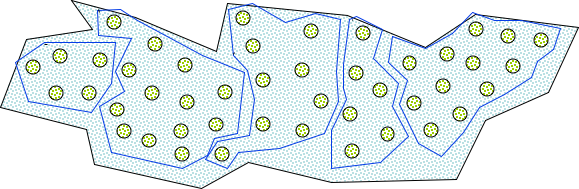
\includegraphics[scale=0.5]{../Figures/CompleteCoveragePrinciple.png}

\end{frame}

%%%%%%%%%%%%%%%%%%%%%%%%%%%%%%%%%%%%%%%%%%%%%%%%%%%%%%

\begin{frame}
\frametitle{White-box Testing}

\begin{itemize}
\item \structure{Intuitively, after running your test suites, what percentage of
    the lines of code in your program should be exercised?}
\end{itemize}

\end{frame}

%%%%%%%%%%%%%%%%%%%%%%%%%%%%%%%%%%%%%%%%%%%%%%%%%%%%%%

\begin{frame}
\frametitle{White-box Coverage Testing}

\begin{itemize}
\item (In)adequacy criteria - if significant parts of the program structure are not tested, testing is inadequate
\item Control flow coverage criteria
\begin{itemize}
\item Statement coverage
\item Edge coverage
\item Condition coverage
\item Path coverage
\end{itemize}
\end{itemize}
Examples that follow are from \cite{GhezziEtAl2003}
\end{frame}

%%%%%%%%%%%%%%%%%%%%%%%%%%%%%%%%%%%%%%%%%%%%%%%%%%%%%%

\begin{frame}
\frametitle{Statement-Coverage Criterion}

\begin{itemize}
\item Select a test set $T$ such that every elementary statement in $P$ is
  executed at least once by some $d$ in $T$
\item An input datum executes many statements - try to minimize the number of
  test cases still preserving the desired coverage
\end{itemize}

\end{frame}

%%%%%%%%%%%%%%%%%%%%%%%%%%%%%%%%%%%%%%%%%%%%%%%%%%%%%%

\begin{frame}
\frametitle{Example}

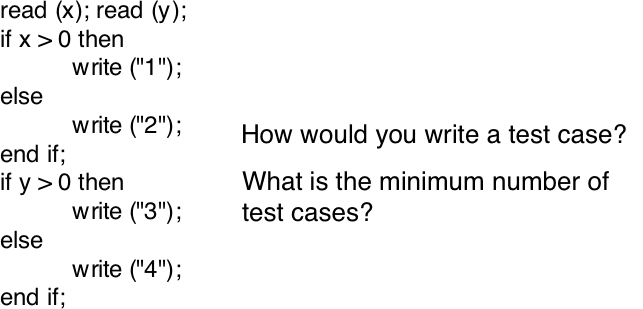
\includegraphics[scale=0.5]{../Figures/ExampleStatementCoverageOnlyCode.png}

\end{frame}

%%%%%%%%%%%%%%%%%%%%%%%%%%%%%%%%%%%%%%%%%%%%%%%%%%%%%%

\begin{frame}
\frametitle{Example}

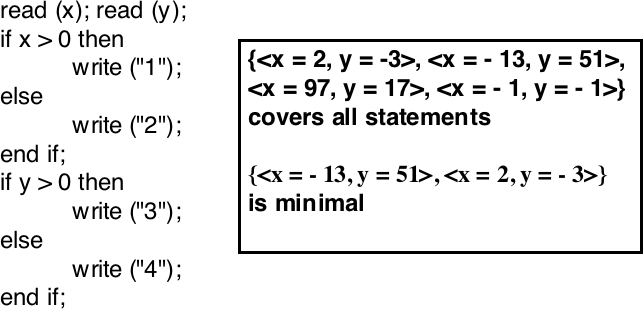
\includegraphics[scale=0.5]{../Figures/ExampleStatementCoverage.png}

\end{frame}

%%%%%%%%%%%%%%%%%%%%%%%%%%%%%%%%%%%%%%%%%%%%%%%%%%%%%%

\begin{frame}
\frametitle{Weakness of the Criterion}

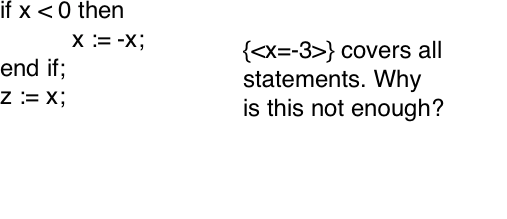
\includegraphics[scale=0.6]{../Figures/WeaknessStatementCoverageOnlyCode.png}

\end{frame}

%%%%%%%%%%%%%%%%%%%%%%%%%%%%%%%%%%%%%%%%%%%%%%%%%%%%%%

\begin{frame}
\frametitle{Weakness of the Criterion}

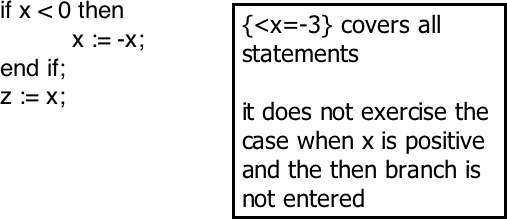
\includegraphics[scale=0.6]{../Figures/WeaknessStatementCoverage.png}

\end{frame}

%%%%%%%%%%%%%%%%%%%%%%%%%%%%%%%%%%%%%%%%%%%%%%%%%%%%%%

\begin{frame}
\frametitle{Edge-Coverage Criterion}

\begin{itemize}
\item Select a test set $T$ such that every edge (branch) of the control flow is
  exercised at least once by some $d$ in $T$
\item This requires formalizing the concept of the control graph and how to construct it
\begin{itemize}
\item Edges represent statements
\item Nodes at the ends of an edge represent entry into the statement and exit
\end{itemize}
\end{itemize}

\end{frame}

%%%%%%%%%%%%%%%%%%%%%%%%%%%%%%%%%%%%%%%%%%%%%%%%%%%%%%

\begin{frame}
\frametitle{Control Graph Construction Rules}

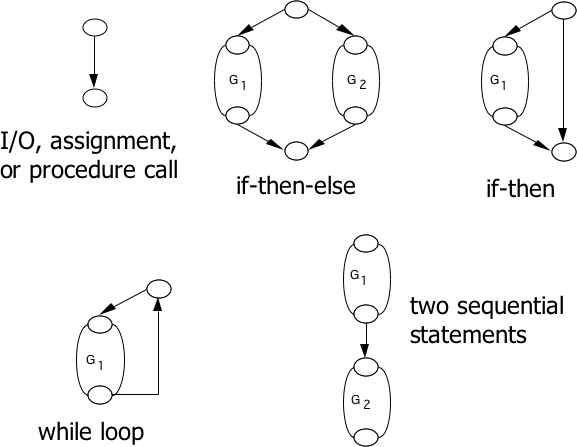
\includegraphics[scale=0.4]{../Figures/ControlGraphRules.png}

\end{frame}

%%%%%%%%%%%%%%%%%%%%%%%%%%%%%%%%%%%%%%%%%%%%%%%%%%%%%%

\begin{frame}
\frametitle{Simplification}

A sequence of edges can be collapsed into just one edge\\
~\newline

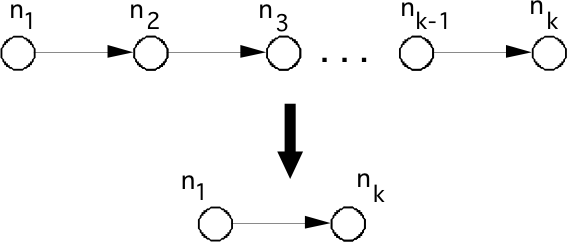
\includegraphics[scale=0.5]{../Figures/Simplification.png}

\end{frame}

%%%%%%%%%%%%%%%%%%%%%%%%%%%%%%%%%%%%%%%%%%%%%%%%%%%%%%

\begin{frame}
\frametitle{Example: Euclid's Algorithm}

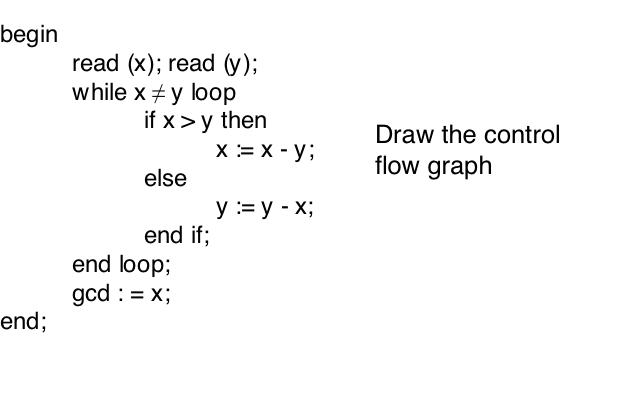
\includegraphics[scale=0.5]{../Figures/EuclidsAlgorithmNoGraph.png}

\end{frame}

%%%%%%%%%%%%%%%%%%%%%%%%%%%%%%%%%%%%%%%%%%%%%%%%%%%%%%

\begin{frame}
\frametitle{Example: Euclid's Algorithm}

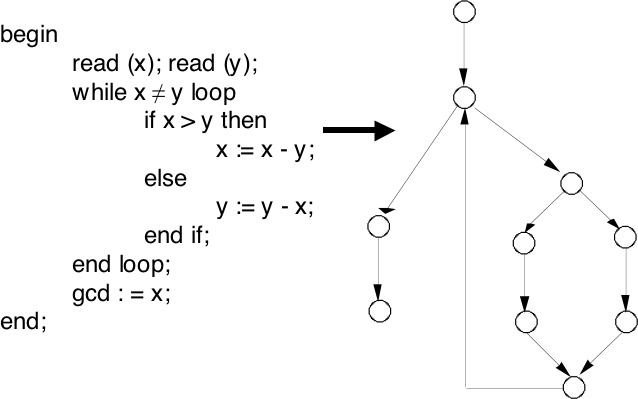
\includegraphics[scale=0.5]{../Figures/EuclidsAlgorithm.png}

\end{frame}

%%%%%%%%%%%%%%%%%%%%%%%%%%%%%%%%%%%%%%%%%%%%%%%%%%%%%%

\begin{frame}
\frametitle{Weakness}

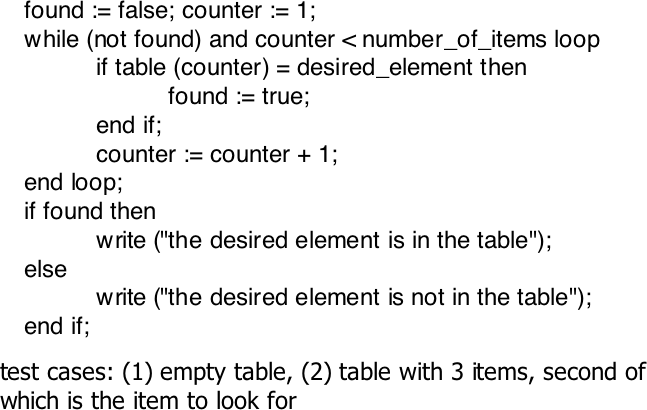
\includegraphics[scale=0.4]{../Figures/WeaknessEdgeCoverage.png}\\
\uncover<2->{\structure{Do not discover the error ($<$ instead of $\leq$)}}

\end{frame}

%%%%%%%%%%%%%%%%%%%%%%%%%%%%%%%%%%%%%%%%%%%%%%%%%%%%%%

\begin{frame}
%\frametitle{Alternative View of Condition Coverage}

\lstset{language=java,breaklines=true,showspaces=false,showstringspaces=false,breakatwhitespace=true}
\noindent \lstinputlisting{CondCovExample.java}

\end{frame}

%%%%%%%%%%%%%%%%%%%%%%%%%%%%%%%%%%%%%%%%%%%%%%%%%%%%%%

\begin{frame}
\frametitle{Condition-Coverage Criterion}

\begin{itemize}
\item Select a test set $T$ such that every edge of $P$'s control flow is traversed and all possible values of the
constituents of compound conditions are exercised at least once
\item This criterion is finer than edge coverage
\end{itemize}

\end{frame}

%%%%%%%%%%%%%%%%%%%%%%%%%%%%%%%%%%%%%%%%%%%%%%%%%%%%%%

\begin{frame}
\frametitle{Weakness}

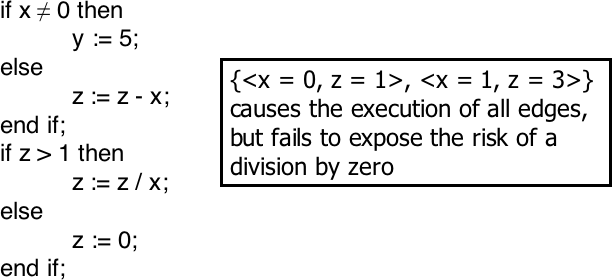
\includegraphics[scale=0.5]{../Figures/WeaknessConditionCoverage.png}

\end{frame}

%%%%%%%%%%%%%%%%%%%%%%%%%%%%%%%%%%%%%%%%%%%%%%%%%%%%%%

\begin{frame}
\frametitle{Path-Coverage Criterion}

\begin{itemize}
\item Select a test set $T$ that traverses all paths from the initial to the final node of $P$s control flow
\item It is finer than the previous kinds of coverage
\item However, number of paths may be too large, or even infinite (see while loops)
\item Loops
\begin{itemize}
\item Zero times (or minimum number of times)
\item Maximum times
\item Average number of times
\end{itemize}
\end{itemize}

\end{frame}

%%%%%%%%%%%%%%%%%%%%%%%%%%%%%%%%%%%%%%%%%%%%%%%%%%%%%%

\begin{frame}
\frametitle{The Infeasibility Problem}

\begin{itemize}
\item Syntactically indicated behaviours (statements, edges, etc.) are often impossible
\item Unreachable code, infeasible edges, paths, etc.
\item Adequacy criteria may be impossible to satisfy
\begin{itemize}
\item Manual justification for omitting each impossible test case
\item Adequacy ``scores'' based on coverage - example 95 \% statement coverage
\end{itemize}
\end{itemize}

\end{frame}

%%%%%%%%%%%%%%%%%%%%%%%%%%%%%%%%%%%%%%%%%%%%%%%%%%%%%%

\begin{frame}
\frametitle{Further Problem}

\begin{itemize}
\item What if the code omits the implementation of some part of the specification?
\item White box test cases derived from the code will ignore that part of the specification!
\end{itemize}

\end{frame}

%%%%%%%%%%%%%%%%%%%%%%%%%%%%%%%%%%%%%%%%%%%%%%%%%%%%%%

\begin{frame}
\frametitle{Testing Boundary Conditions}

\begin{itemize}

\item Testing criteria partition input domain in classes, assuming that behavior
  is ``similar'' for all data within a class
\item Some typical programming errors, however, just happen to be at the
  boundary between different classes
\begin{itemize}
\item Off by one errors
\item $<$ instead of $\leq$
\item equals zero
\end{itemize}
\end{itemize}

\end{frame}

%%%%%%%%%%%%%%%%%%%%%%%%%%%%%%%%%%%%%%%%%%%%%%%%%%%%%%

\begin{frame}
\frametitle{Criterion}

\begin{itemize}

\item After partitioning the input domain D into several classes, test the
  program using input values not only ``inside'' the classes, but also at their
  boundaries
\item This applies to both white-box and black-box techniques
\item In practice, use the different testing criteria in combinations
\item Use testing tools for coverage metrics
\end{itemize}

\end{frame}

%%%%%%%%%%%%%%%%%%%%%%%%%%%%%%%%%%%%%%%%%%%%%%%%%%%%%%

\begin{frame}
\frametitle{The Oracle Problem}

\structure{When might it be difficult to know the ``expected''
  output/behaviour?}

\end{frame}

%%%%%%%%%%%%%%%%%%%%%%%%%%%%%%%%%%%%%%%%%%%%%%%%%%%%%%

\begin{frame}
\frametitle{The Oracle Problem}

\begin{itemize}

\item Given input test cases that cover the domain, what are the expected
  outputs?
\item Oracles are required at each stage of testing to tell us what the right
  answer is
\item Black-box criteria are better than white-box for building test oracles
\item Automated test oracles are required for running large amounts of tests
\item Oracles are difficult to design - no universal recipe
\end{itemize}

\end{frame}

%%%%%%%%%%%%%%%%%%%%%%%%%%%%%%%%%%%%%%%%%%%%%%%%%%%%%%

\begin{frame}
\frametitle{The Oracle Problem Continued}

\begin{itemize}

\item Determining what the right answer should be is not always easy
\begin{itemize}
%\item Air traffic control system
\item Scientific computing
\item Machine learning
\item Artifical intelligence
\end{itemize}
\end{itemize}

\end{frame}

%%%%%%%%%%%%%%%%%%%%%%%%%%%%%%%%%%%%%%%%%%%%%%%%%%%%%%

\begin{frame}
\frametitle{The Oracle Problem Continued}

\structure{What are some strategies we can use when we do not have a test
  oracle?}

\end{frame}

%%%%%%%%%%%%%%%%%%%%%%%%%%%%%%%%%%%%%%%%%%%%%%%%%%%%%%

\begin{frame}
\frametitle{Strategies Without An Oracle}

\begin{itemize}

\item Using an independent program to approximate the oracle (pseudo oracle)
\item Method of manufactured solutions
\item Properties of the expected values can be easier than stating the expected
  output
\bi
\item \uncover<1->{\structure<1>{Examples?}}
\item \uncover<2->{List is sorted}
\item \uncover<2->{Number of entries in file matches number of inputs}
\item \uncover<2->{Conservation of energy or mass}
\item \uncover<2->{Expected trends in output are observed (metamorphic testing
    \cite{Kanewala2015, KanewalaAndBieman2013, KanewalaAndLundgren2016})}
\item \uncover<2->{etc.}
\ei
\end{itemize}

\end{frame}

%%%%%%%%%%%%%%%%%%%%%%%%%%%%%%%%%%%%%%%%%%%%%%%%%%%%%%

% \begin{frame}
% \frametitle{Analysis of Units}
% \begin{itemize}
% \item Dynamic testing of units is not the only option
% \item Static testing (analysis) includes the following
% \begin{itemize}
% \item Informal inspection
% \item Systematic inspection
% \item Code walkthroughs, data flow analysis
% \item Correctness proofs (for instance using pre and post conditions)
% \item Complexity measures
% \end{itemize}
% \end{itemize}
% \end{frame}

%%%%%%%%%%%%%%%%%%%%%%%%%%%%%%%%%%%%%%%%%%%%%%%%%%%%%%%%%%%%%%%%%%%%%%%%%%%%%

\begin{frame}
\frametitle{Challenges Specific to Scientific Computing}
\begin{itemize}
\item Unknown solution
\item Approximation of real numbers
\item Nonfunctional requirements
\item Parallel computation
\end{itemize}
\end{frame}

%%%%%%%%%%%%%%%%%%%%%%%%%%%%%%%%%%%%%%%%%%%%%%%%%%%%%%%%%%%%%%%%%%%%%%%%%%%%%

\begin{frame}
\frametitle{Mutation Testing for SC}
\begin{itemize}
\item Generate changes to the source code, called mutants, which become code faults
\item Mutants include changing an operation, modifying constants, changing the order of execution, etc.
\item The adequacy of a set of tests is established by running the tests on all generated mutants
\item Need to account for floating point approximations
\item See \cite{HookAndKelly2009}
\end{itemize}
\end{frame}

%%%%%%%%%%%%%%%%%%%%%%%%%%%%%%%%%%%%%%%%%%%%%%%%%%%%%%%%%%%%%%%%%%%%%%%%%%%%%

\begin{frame}
\frametitle{Specific SC V\&V Approaches}
Summary of most points below in \cite{Smith2016}
\begin{itemize}
\item Compare to closed-form solutions
\item Method of manufactured solutions \cite{Roache1998}
\item Interval arithmetic \cite{Hickey2001}
\item Convergence studies
\item Compare to other program (parallel testing)
\item Can also consider using code inspection
\bi
\item \cite{KellyAndShepard2000,
  ShepardAndKelly2001}
\item \href{http://www.cs.nott.ac.uk/~pszcah/G53QAT/fi.pdf}{Sample checklists}
\ei
\end{itemize}
\end{frame}

%%%%%%%%%%%%%%%%%%%%%%%%%%%%%%%%%%%%%%%%%%%%%%%%%%%%%%%%%%%%%%%%%%%%%%%%%%%%%

\begin{frame}
\frametitle{Specific SC V\&V NonFunctional}

\begin{itemize}
\item Installability, consider VMs
\item Portability, consider VMs, Docker, CI
\item Describe (rather than specify) impact of changing inputs
\bi
\item Accuracy
\item Performance
\item Relative comparison
\ei
\item Usability
\bi
\item \href{https://measuringu.com/sus/}{Fairly simple standard survey}
\item \href{https://gitlab.cas.mcmaster.ca/andrem5/RogueReborn/blob/master/Doc/TestPlan/TestPlan.pdf}{Example}
\ei
\end{itemize}
\end{frame}

%%%%%%%%%%%%%%%%%%%%%%%%%%%%%%%%%%%%%%%%%%%%%%%%%%%%%%%%%%%%%%%%%%%%%%%%%%%%%

\begin{frame}
\frametitle{Validation Testing Report for PMGT}
\begin{itemize}
\item Prepared by Wen Yu (\href{https://gitlab.cas.mcmaster.ca/smiths/cas741/blob/master/Examples/MeshGenToolbox/doc/testingApp.pdf}{here})
\item Do not know the correct solution, but know properties of the correct solution
\item Automated correctness validation tests
\begin{itemize}
\item The area of each element is greater than zero
\item The boundary of the mesh is closed
\item Vertices in a clockwise order
\item $nc + nv - ne = 1$
\item ...
\end{itemize}
\item Visual correctness verification tests
\begin{itemize}
\item No vertex outside the input domain
\item No vertex inside a cell
\item No dangling edges
\item All cells connected
\item  The mesh is conformal
\end{itemize}
\end{itemize}
\end{frame}

%%%%%%%%%%%%%%%%%%%%%%%%%%%%%%%%%%%%%%%%%%%%%%%%%%%%%%%%%%%%%%%%%%%%%%%%%%%%%

\begin{frame}
\frametitle{Validation Testing Report for PMGT (Continued)}
\begin{itemize}
\item List and description of test cases
\item Test cases are labelled and numbered
\item Traceability to SRS requirements
\item Traceability to MG
\item Summary of results
\item Analysis of results
\begin{itemize}
\item Focus on nonfunctional requirements
\item Speed
\end{itemize}
\end{itemize}
\end{frame}

%%%%%%%%%%%%%%%%%%%%%%%%%%%%%%%%%%%%%%%%%%%%%%%%%%%%%%%%%%%%%%%%%%%%%%%%%%%%%

\begin{frame}
  \frametitle{Test Plan From BlankProjectTemplate}

  \begin{itemize}
  \item Add links to templates
  \item For Unit VnV plan mention tools
    \begin{itemize}
    \item Linters
    \item Coding standard checkers (like flake8)
    \item unit testing frameworks
    \item Performance testing (like Valgrind)
    \end{itemize}
  \end{itemize}
\end{frame}

%%%%%%%%%%%%%%%%%%%%%%%%%%%%%%%%%%%%%%%%%%%%%%%%%%%%%%%%%%%%%%%%%%%%%%%%%%%%%

\begin{frame}[allowframebreaks]
\frametitle{References}

\bibliography{../../ReferenceMaterial/References}

\end{frame}

%%%%%%%%%%%%%%%%%%%%%%%%%%%%%%%%%%%%%%%%%%%%%%%%%%%%%%

\end{document}